 \documentclass[book.tex]{subfiles}
\begin{document}

The original Commander Keen, Commander Keen in Invasion of the Vorticons, was only released for the EGA videocard. Keen Dreams and later versions included a CGA version as well. The game play was exactly the same, sounds were the same, it was just that the graphics were CGA. Before diving into  the source code, let's first get a better understanding of the CGA video hardware.\\


\begin{figure}[H] 
  \centering 
  \scaledimage{1.0}{game/Keen_EGA_CGA.png} 
  \caption{Keen Dreams EGA and CGA version.}
\end{figure}

\par
\textbf{\underline{Trivia :}} It's an ironic twist that Softdisk did not use the original Keen's engine, as the code violated the company policy by depending on 16-color EGA hardware without supporting older 4-color CGA cards!\\
\par


 

\section{CGA Videocard}
The Color Graphics Adapter (CGA), originally also called the Color/Graphics Adapter or IBM Color/Graphics Monitor Adapter, introduced in 1981, was IBM's first color graphics card for the IBM XT.\\
\par
The CGA card can be summarized by the following hardware:
\begin{itemize}
  \item It was built around the Motorola 6845 display controller.
  \item The framebuffer (the VRAM) contained two memory banks of 8 kilobytes each, resulting in 16 kilobytes total.
  \item Character generator ROM, containing a 14-row font and two 8x8 fonts. This is the same ROM as used on the MDA videocard.
\end{itemize}

\begin{figure}[H] 
  \centering 
  \scaledimage{1.0}{hardware/IBM-CGA.jpg} 
  \caption{The CGA is a full-length 8-bit ISA card.}
\end{figure}

The CGA card has the following text and graphics modes:\\
\vspace{-10pt}
\begin{figure}[H]
\centering
\begin{table}[H]
\begin{tabularx}{\textwidth}[c]{llllcr}
\hline
\textbf{Mode} & \textbf{Type} & \textbf{Format} & \textbf{Colors} & \hspace{10pt}\textbf{RAM Mapping}\hspace{10pt} & \textbf{Hz}        \\ \hline
0             & text          & 40x25           & 16 (monochrome) & B8000h     & 60                           \\ \hline
1             & text          & 40x25           & 16              & B8000h    & 60                            \\ \hline
2             & text          & 80x25           & 16 (monochrome) & B8000h    & 60                            \\ \hline
3             & text          & 80x25           & 16              & B8000h    & 60                            \\ \hline
4             & CGA Graphics  & 320x200         & 4               & B8000h    & 60                            \\ \hline
5             & CGA Graphics  & 320x200         & 4 (monochrome)  & B8000h    & 60                            \\ \hline
6             & CGA Graphics  & 640x200         & 2               & B8000h    & 60                            \\ \hline

\end{tabularx}
\end{table}
\caption{EGA Modes available.}
\label{ega-modes-available}
 \end{figure} 

In the graphics mode 4, which is used by Commander Keen, each pixel is using 2 bits for color, resulting in only four colors being displayed at a time. These four colors could not be freely chosen from the 16 CGA colors, there were only two official palettes for this mode:
\begin{enumerate}
  \item Magenta, cyan, white and background colour (black by default).
  \item Red, green, brown/yellow and background colour (black by default).
\end{enumerate}
The background color could be any of the 16 colors, but often it was kept black. For each mode there is a high- and low-intensity version of the palette.\\

\begin{figure}[H]
\centering
\begin{table}[H]
\begin{tabularx}{\textwidth}[c]{|>{\hsize=.24\hsize}X |>{\hsize=.24\hsize}X |>{\hsize=.24\hsize}X |>{\hsize=.28\hsize}X |}
\hline
\multicolumn{2}{|c|}{\textbf{\color{black}Palette 1}} & \multicolumn{2}{|c|}{\textbf{\color{black}Palette 2}} 	\\ 
\hline
\textbf{\color{black} low intensity} & \textbf{\color{black} high intensity} & \textbf{\color{black} low intensity} & \textbf{\color{black} high intensity} \\
\color{white}\cellcolor{CGA_Black}0 - Background & \color{white}\cellcolor{CGA_Black} - Background &\color{white}\cellcolor{CGA_Black}0 - Background & \color{white}\cellcolor{CGA_Black}0 - Background \\

\color{black}\cellcolor{CGA_Green}2 - Green & \color{black}\cellcolor{CGA_Bright_Green}10 - Bright Green &\color{black}\cellcolor{CGA_Cyan}3 - Cyan & \color{black}\cellcolor{CGA_Bright_Cyan}11 - Bright Cyan \\

\color{black}\cellcolor{CGA_Red}4 - Red & \color{black}\cellcolor{CGA_Bright_Red}12 - Bright Red &\color{black}\cellcolor{CGA_Magenta}5 - Magenta & \color{black}\cellcolor{CGA_Bright_Magenta}13 - Bright Magenta \\

\color{black}\cellcolor{CGA_Brown}6 - Brown & \color{black}\cellcolor{CGA_Bright_Brown}14 - Yellow &\color{black}\cellcolor{CGA_Light_Grey}7 - Bright Grey & \color{black}\cellcolor{CGA_White}15 - White \\
\hline

\end{tabularx}
\end{table}
\caption{CGA color palettes.}
\label{default_ega_palette}
 \end{figure}
 
The default palette when switching to Mode \cw{04h} is palette 2 with high intensity, which is used by Commander Keen.  


\section{Memory architecture and Interlacing}
 
The CGA memory layout in graphics mode is different compared to EGA, as it is based on interlaced architecture.
Normally, video memory is strictly linear: the next row of display data corresponds to the next row of pixels. But with CGA, the next row of display data corresponded to the row of pixels two rows down. This continued until the end of the screen and only with the second half of display data were the in-between rows addressed. So VRAM bank 0 was for even rows 0, 2, 4, etc., until the end of the screen and VRAM bank 1 was for odd rows 1, 3, 5, etc. This added calculation steps to most CGA graphics operations if the programmer wanted to avoid visual artifacts when updating the screen.\\
\par
Each pair of 2 bits is one pixel with a color value of 0-3, referring to the CGA color palette. The 2 most left bits represent pixel 0, the next 2 bits pixel 1, etc. So each byte in VRAM represents 4 pixels on screen. \\






\begin{figure}[H]
\centering
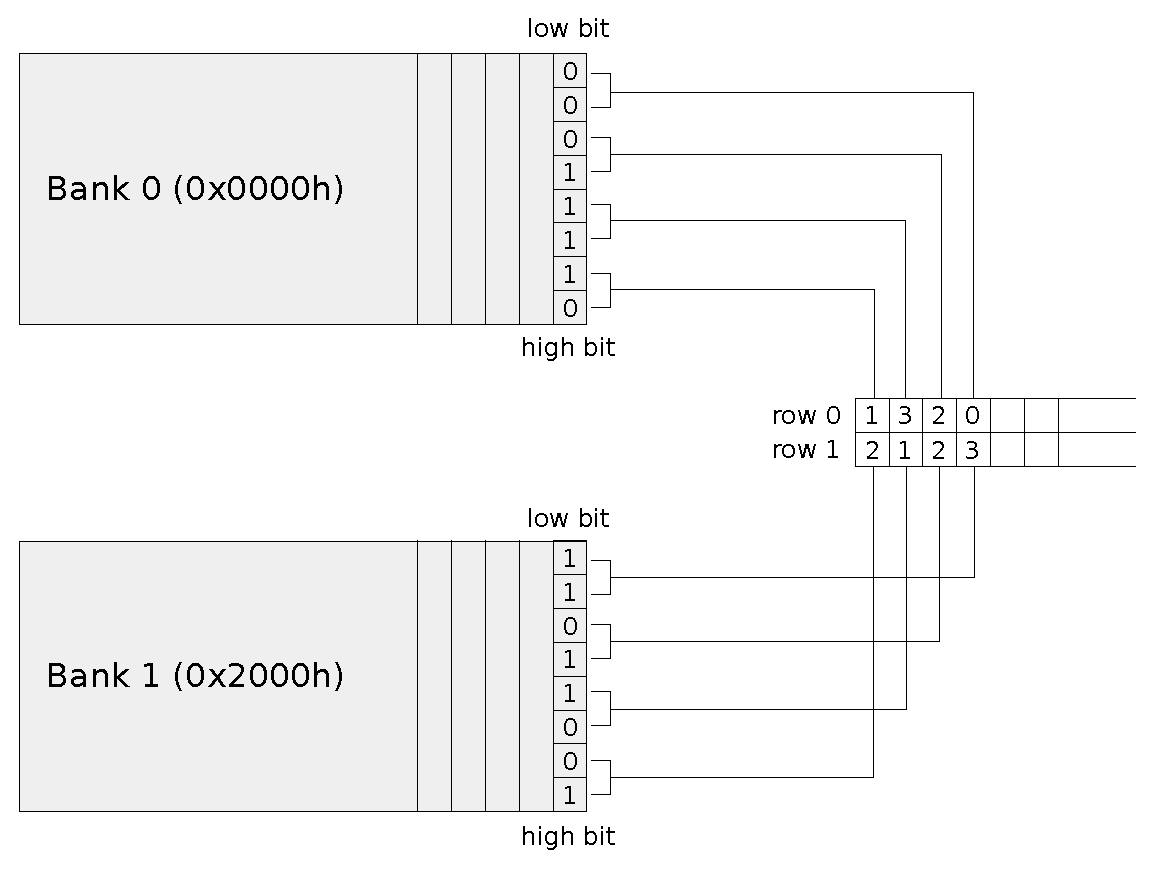
\includegraphics[width=1.0\textwidth]{imgs/drawings/cga_interlace.eps}
\caption{CGA interlaced memory.}
\label{fig:cga_interlaced}
\end{figure}


\par
The CGA card is making use of memory mapping, just like EGA. In mode \cw{04h}, the VRAM bank 0 is mapped from 0xB0000 to 0xB1FFF and VRAM bank 1 is mapped from 0xB2000 to 0xB3FFF. Unlike EGA, the CGA memory model doesn't require masking as the total 16KiB VRAM fits easy in a 64KiB memory segment.\\ 

\par
\textbf{\underline{Trivia :}} Interesting enough, interlacing is never really implemented in CGA. When displaying the VRAM to screen it does a progressive (lineair) scan, where it alternately reads from bank 0 and bank 1.\\
\par


\section{Double buffering}
A full picture in mode \cw{04h} requires 320 pixels * 2 bits per pixel * 200 lines = 16,000 bytes of memory. This means the display screen requires all 16KiB memory and there is no capacity in VRAM for extra screens. The only way to introduce double buffering on CGA is by creating a 64 KiB buffer in conventional memory.  \\
\par
\begin{minipage}{\textwidth}
  \lstinputlisting[language=C]{code/cga_init_buffer.c}
\end{minipage}
\label{state_type}
\par
The memory buffer contains both the buffer page and the static master page, each has a logical with of 512 pixels wide. The buffer page starts at offset \cw{0x0000h} and the master page start at \cw{0x8000h}. Both pages float around in the 64KiB memory segment, making use of the same memory wrapping as explained in section \ref{section:wrap_ega_memory}.


\begin{figure}[H]
\centering
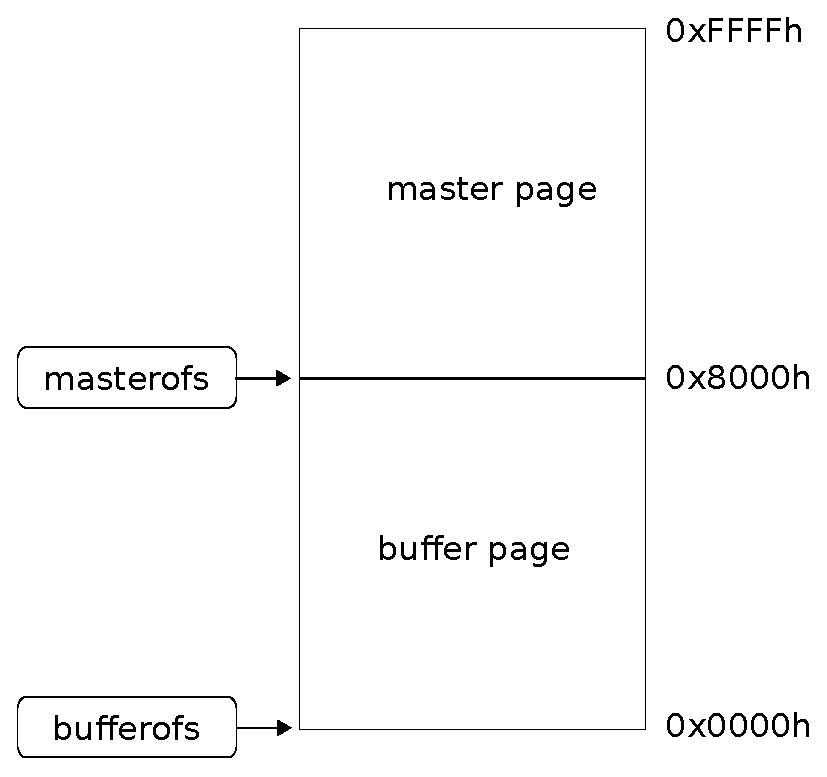
\includegraphics[width=0.6\textwidth]{imgs/drawings/cga_screenseg.eps}
\caption{CGA double buffering memory layout.}
\label{fig:cga_screenseg}
\end{figure}

\section{Screen refresh}
With the double buffering in place, the same algoritm as implemented for EGA can be used. The final step of the algoritm is updating the screen display by copying the buffer page to the VRAM. However, there are two complications with CGA.\\

\par
The first complication is that the CGA card does not support pixel panning. So the smoothest pixel scroll is equal to scroll the screen with one byte. Since one byte represents 4 pixels, it means scrolling to left or right is in steps of 4 pixels.\\

\begin{figure}[H]
\centering
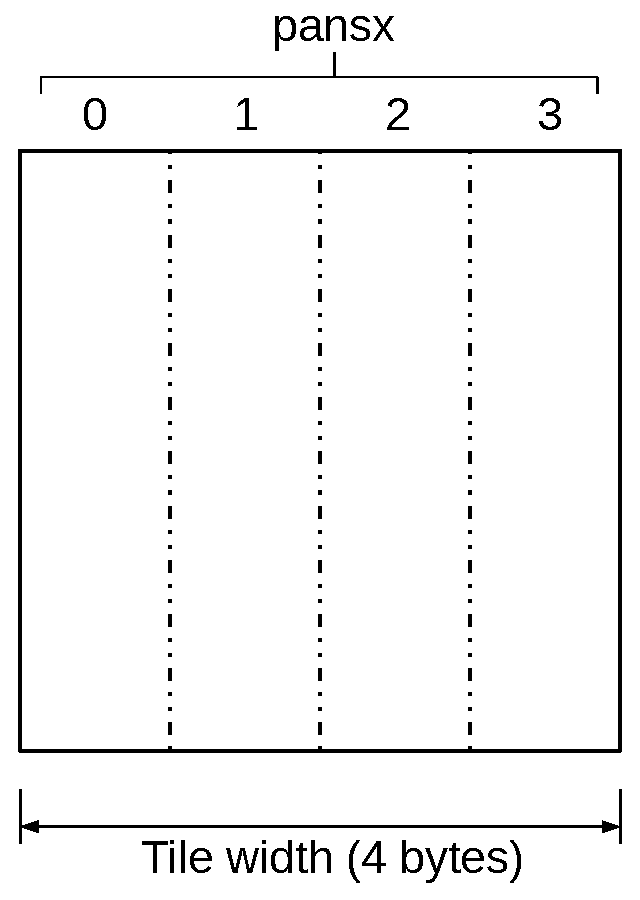
\includegraphics[width=0.3\textwidth]{imgs/drawings/CGA_Tile_Refresh.eps}
\label{fig:cga_tile_panning}
\end{figure}

\par
\begin{minipage}{\textwidth}
  \lstinputlisting[language=C]{code/cga_calc_origin.c}
\end{minipage}
\label{state_type}
\par

The second complication involves copying the RAM buffer to the interlaced VRAM. This requires to split the lineair memory buffer into copying all even rows to VRAM bank 0 and odd rows to VRAM bank 1.\\

\begin{figure}[H]
\centering
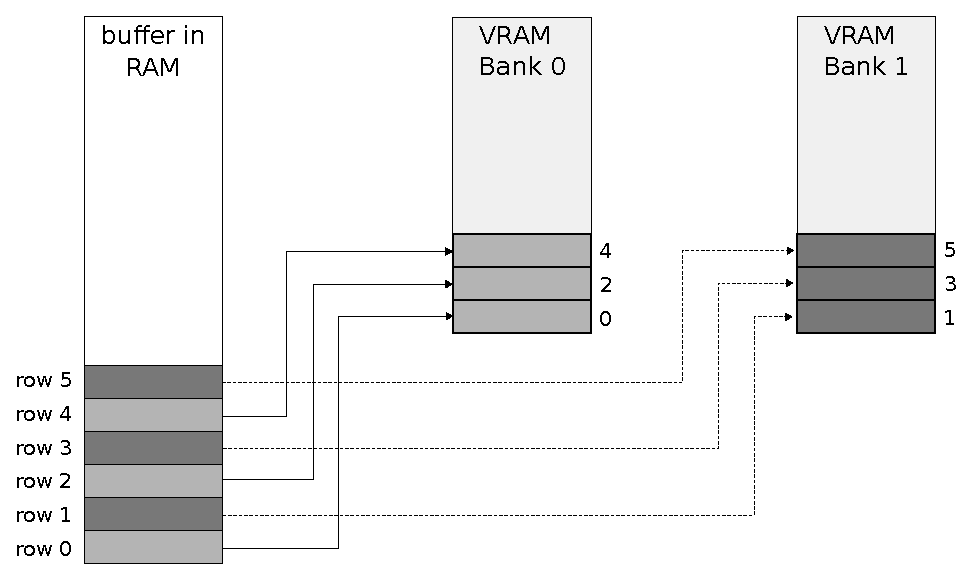
\includegraphics[width=1.0\textwidth]{imgs/drawings/cga_VRAM_copy.eps}
\caption{CGA memory to VRAM copy.}
\label{fig:cga_interlaced}
\end{figure}

\par
To avoid screen tearing the system should wait for a vertical retrace, like it was done with EGA. The problem is that computers weren't fast enough to copy all bytes from RAM buffer to VRAM during the vertical retrace period. So in the CGA version of Commander Keen, it was not possible to avoid screen tearing.\\

\par
\begin{minipage}{\textwidth}
  \lstinputlisting[language=C]{code/cga_screen_refresh.c}
\end{minipage}
\label{cga_screen_refresh}
\par

\par
The original IBM CGA card could not handle writing and reading VRAM at the same time. Because video memory on the IBM CGA isn't dual-ported, when the CPU and the video card need access to the same byte of video RAM, the CPU wins; the card ends up reading a random value, causing "snow" on the screen. The only way to avoid the snow was, also in the case, to wait for the vertical retrace. Most CGA clones resolved the issue by enabling read/write VRAM at the same time, but if one would play Commander Keen on the original IBM CGA card you experience both screen tearing and snow.\\
\par

\end{document}